\documentclass{article}

\usepackage{multicol}
\usepackage{graphicx}
\usepackage{caption}
\usepackage[left=2cm,right=2cm,top=2cm,bottom=2.5cm]{geometry}

\title{\textbf{MATH 300 Final Project}}
\author{Ali Hamza $|$ Maham Shoaib $|$ Hassan Naseem}
\date{\today}

\begin{document}
\maketitle

\section{Tasks}
\subsection{Task 1}
In this task we took a few assumptions to model the 1 dimensional random walk. Since there 
were only 3 possible movements: right, left, or no movement. We chose to model the walk using a 
uniform distribution. This was done by generating an array of random integers from the set $\{1,2,3\}$, similar to 
throwing a 3 sided die.
\begin{itemize}
    \item On 1, the particle moves right 1 unit
    \item On 2, the particle moves left 1 unit
    \item On 3, the particle does not move
\end{itemize}
Upon running the code by varying the number of steps the particle takes the following graphs
were produced.
%Figure (Images of Graphs Obtained)
    \begin{multicols}{3}[\columnsep=3cm]
        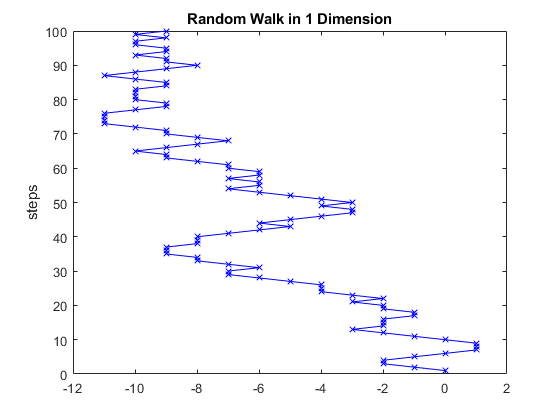
\includegraphics[scale=0.3]{r1d100.png}
        \columnbreak
        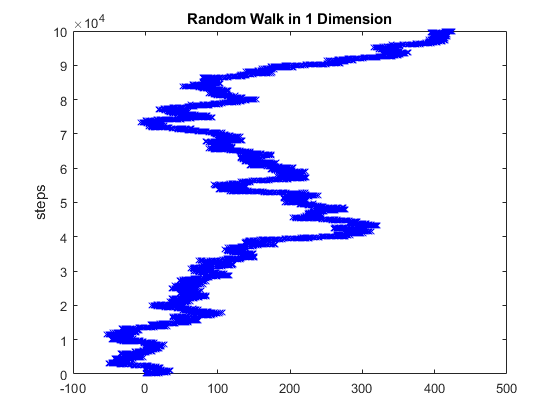
\includegraphics[scale=0.3]{r1d100000.png}
        \columnbreak
        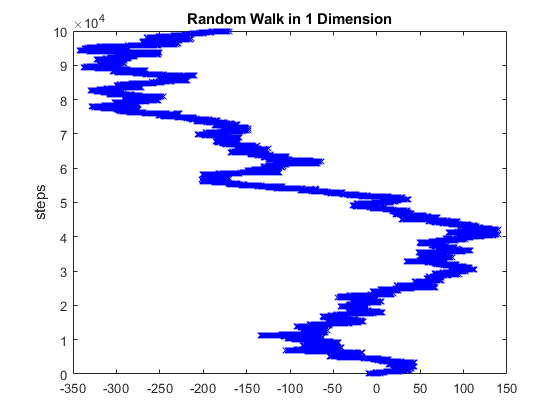
\includegraphics[scale=0.3]{r1d1000000.png}
        \end{multicols}
    \captionof{figure}{Steps = 100, 100000, 1000000 from left to right}

To find the expected average distance from the start we assumed 

\subsection{Task 2}
In this task took the assumption of placing the particles at certain positions. Particle 
A starts of (0) on the x axis and Particle B starts off an $x$ distance away from Particle A, where $x$ is 
a parameter of the function.

\subsection{Task 3}
\subsection{Task 4}
\subsection{Task 5}
\subsection{Task 6}
\subsection{Task 7}
\subsection{Task 8}
\section{Bibliography}

\end{document}